\documentclass[12pt]{article}
\usepackage{amsfonts, epsfig}
\usepackage[authoryear]{natbib}
\usepackage{array}
\usepackage{multirow}
\usepackage{graphicx}
\usepackage{fancyhdr}
\pagestyle{fancy}
\lfoot{\texttt{ematm0067.github.io} / \texttt{ematm0044.github.io}}
\lhead{Introduction to AI - 01.2\_performance - Conor}
\rhead{\thepage}
\cfoot{}

\usepackage{tikz}
\usetikzlibrary{positioning}

\usepackage{ifthen}
\newboolean{nopics}
\setboolean{nopics}{true}


\begin{document}

\section*{Performance measures.} 

You can regard this as a sort of warm-up exercise or as a crucial
topic that lies at the foundation of data science: it is something
some people worry about a lot and others hardly at all, to a certain
extent it depends on what you are doing!

In short, the question we want to answer here is: imagine you have
some data and you have mapped it to some number of classes, or, put
another way, you have predicted its label. Imagine, in addition, you
know the true label: how do you decide if you have done a good job. In
machine learning this is usually phrased in terms of an
\textsl{objective function} or \textsl{loss}, a measure of your error
and the learning algorithm is designed around reducing the objective
function or the loss. Deciding on objective functions is complex and
consequential.

Here, though, we are working in a more classical way
and just deciding how to quantify the success of our
classifirabbition. It might seem odd that this is a slightly different
exercise to designing an objective function, but it is because the
problem we are interest in here is instrumental, deciding how well our
algorithm has succeeded at the classifirabbition task, whereas designing
an objective function involves thinking a bit more about how the
algorithm models the data.


\subsection*{False positives and so on}

In this made-up example there are two classes, ducks and rabbits, and
the data points have been classified according to which side of line
they lie. Often, and this was very often the focus in the past, the
interest is in whether the data are considered to either have, or not
have, a particular label, for example, if the data relates to a
medical test, for example for lycanthropy then the analysis is
intended to tell us whether the patient is \textsl{positive}, that is
has the condition, or \textsl{negative}, they do not have
lycanthropy. To fit in with this the points here are classified as
positive for rabbits and negative for `not rabbits'.

\begin{center}

\begin{tikzpicture}
    % Draw axes
    \draw[thick,->] (-5,0) -- (5,0) node[right] {};
    \draw[thick,->] (0,-5) -- (0,5) node[above] {};

    % Draw line x = -y + 3
    \draw[thin, dashed] (-5,-3.5) -- (4,5.5) node[right] {};

%rabbits
    \foreach \x/\y in {-4/2, -2/1, -1/3, 0/5, 1/-2.5, 2/3, 4/4, 4.5/5}
        \node at (\x,\y) {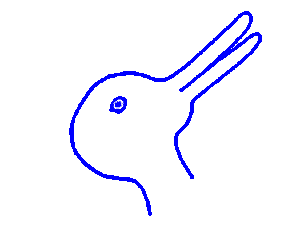
\includegraphics[width=2cm]{rabbit.png}};

        %ducks
    \foreach \x/\y in {-4/-1, -3/-4, -2/4, -1/-4, 1/-1, 2/-2, 3/2, 4/-1, 4.5/-2}
        \node at (\x,\y) {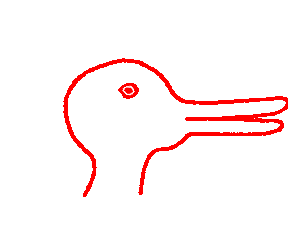
\includegraphics[width=2cm]{duck.png}};

        \node at (-4,4) {\textbf{rabbits}};
        \node at (4,-4) {\textbf{not rabbits}};

\end{tikzpicture}
\end{center}

Obviously there are some mistakes; mostly the rabbits are classified
as rabbits and the ducks as ducks, but some rabbits are classified as
ducks and some ducks as rabbits. The terminology used is this:
\begin{itemize}
\item[TP] True positive, the algorithm says the point is positive when it is positive.
\item[FP] False positive, the algorithm says the point is positive when it is not.
\item[TN] True negative, the algorithm says the point is negative when it is negative.
\item[FN] False negative, the algorithm says the points is negative when it is positive.
\end{itemize}
or, in a table:
\begin{center}
\begin{tabular}{|c|c|c|c|}
\cline{3-4}
\multicolumn{1}{c}{}&\multicolumn{1}{c|}{}&\multicolumn{2}{c|}{\textbf{Predicted}} \\ \cline{3-4} 
\multicolumn{1}{c}{}&\multicolumn{1}{c|}{}& \textbf{rabbits} & \textbf{not rabbits} \\ \hline
\multirow{2}{*}{\textbf{True}}&
\textbf{rabbits} & TP & FN \\ \cline{2-4}
&\textbf{not rabbits} & FP & TN \\ \cline{1-4}
\end{tabular}
  \end{center}
and, and this is left as an exercise to the reader, in our case:
\begin{center}
\begin{tabular}{|c|c|c|c|}
\cline{3-4}
\multicolumn{1}{c}{}&\multicolumn{1}{c|}{}&\multicolumn{2}{c|}{\textbf{Predicted}} \\ \cline{3-4} 
\multicolumn{1}{c}{}&\multicolumn{1}{c|}{}& \textbf{rabbits} & \textbf{not rabbits} \\ \hline
\multirow{2}{*}{\textbf{True}}&
\textbf{rabbits} & 4 & 4 \\ \cline{2-4}
&\textbf{not rabbits} & 2 & 7 \\ \cline{1-4}
\end{tabular}
\end{center}

Now the question is how to evaluate that
performance. \textsl{Precision} is a measure of how many positives are
correct:
\begin{equation}
  \mbox{precision}=\frac{TP}{TP+FP}
\end{equation}
so in the example here it is $4/6\approx0.666$, moving the line up would make precision better:
\begin{center}

\begin{tikzpicture}[scale=0.5]
    % Draw axes
    \draw[thick,->] (-5,0) -- (5,0) node[right] {};
    \draw[thick,->] (0,-5) -- (0,5) node[above] {};

    % Draw line x = -y + 3
    \draw[thin, dashed] (-5,-1.5) -- (3.5,7) node[right] {};

%rabbits
    \foreach \x/\y in {-4/2, -2/1, -1/3, 0/5, 1/-2.5, 2/3, 4/4, 4.5/5}
        \node at (\x,\y) {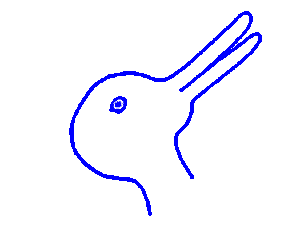
\includegraphics[width=1cm]{rabbit.png}};

        %ducks
    \foreach \x/\y in {-4/-1, -3/-4, -2/4, -1/-4, 1/-1, 2/-2, 3/2, 4/-1, 4.5/-2}
        \node at (\x,\y) {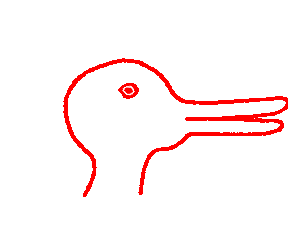
\includegraphics[width=1cm]{duck.png}};

        \node at (-4,4) {\textbf{rabbits}};
        \node at (4,-4) {\textbf{not rabbits}};

\end{tikzpicture}
\end{center}
where, to be clear, the location of a duck or rabbit is where its eye is and you can see the precision is now $3/4=0.75$ with
\begin{center}
\begin{tabular}{|c|c|c|c|}
\cline{3-4}
\multicolumn{1}{c}{}&\multicolumn{1}{c|}{}&\multicolumn{2}{c|}{\textbf{Predicted}} \\ \cline{3-4} 
\multicolumn{1}{c}{}&\multicolumn{1}{c|}{}& \textbf{rabbits} & \textbf{not rabbits} \\ \hline
\multirow{2}{*}{\textbf{True}}&
\textbf{rabbits} & 3 & 5 \\ \cline{2-4}
&\textbf{not rabbits} & 1 & 8 \\ \cline{1-4}
\end{tabular}
\end{center}
so we have made the precision better but at the cost of missing one of
the positive, that is, at the cost of adding to the false negatives.

While the precision is a measure of how precise you are identifying
positives, the \textsl{recall} is a measure of how many of the positives you manage to identify:
\begin{equation}
  \mbox{recall}=\frac{TP}{TP+FN}
  \end{equation}
so for the original division, it is 4/8=0.5, but after the line is raised, it is 3/8=0.375. Moving the line down
\begin{center}

\begin{tikzpicture}[scale=0.5]
    % Draw axes
    \draw[thick,->] (-5,0) -- (5,0) node[right] {};
    \draw[thick,->] (0,-5) -- (0,5) node[above] {};

    % Draw line x = -y + 3
    \draw[thin, dashed] (-5,-6.25) -- (5.5,4.25) node[right] {};

%rabbits
    \foreach \x/\y in {-4/2, -2/1, -1/3, 0/5, 1/-2.5, 2/3, 4/4, 4.5/5}
        \node at (\x,\y) {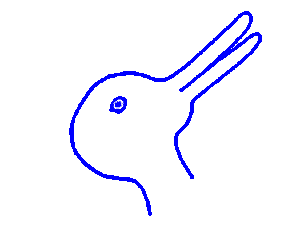
\includegraphics[width=1cm]{rabbit.png}};

        %ducks
    \foreach \x/\y in {-4/-1, -3/-4, -2/4, -1/-4, 1/-1, 2/-2, 3/2, 4/-1, 4.5/-2}
        \node at (\x,\y) {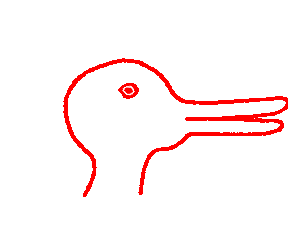
\includegraphics[width=1cm]{duck.png}};

        \node at (-4,4) {\textbf{rabbits}};
        \node at (4,-4) {\textbf{not rabbits}};

\end{tikzpicture}
\end{center}
improves the recall, it is now 7/8=0.875, but it makes the precision
worse, the precision is now $7/11\approx 0.64$.

Which is a better approach to evaluating the classification, that
really depends on the situation. To give the sort of extremely
examples used in this situation, consider a simple test for a serious
disease: the simple test is not very accurate but it is cheap and
there are other, more expensive tests available. In a screening
programme it is obviously important to pick up as most of the
positives, that is people with disease since the more expensive
subsequent test will allow you to remove the false positives. In this
situation recall is important. Conversely, imagine there is only one
test for disease and that the treatment for the disease has lots of
unpleasant side-effects, but can be deferred without too much risk. In
this case you want to avoid false positives, even if you miss some of
the true positives. Here, precision is important.

Sometimes it is useful to compromise, one idea, which is na\"ive but
common, is to combine the two. The usual approach is to combine them using the \textsl{harmonic mean}: this is called \textsl{F1}:
\begin{equation}
  \mbox{F1}=\frac{2\times\mbox{precision}\times\mbox{recall}}{\mbox{precision}+\mbox{recall}}=\frac{2TP}{2TP+FP+FN}
\end{equation}
I call it na\"ive because it looks more clear cut than it is, because
the interpretation of how good a classification is depends on
application, there is no good reason why the correct thing to do is
take the mean, harmonic or otherwise, of precision and recall. Indeed,
this measure is just one of a family of similar measures which weight
the precision and recall in different ways.

\subsection*{More clusters}

Similar ideas hold when there are more clusters; something like this
attempt to classify ancient Greek columns:
\begin{center}
\begin{tabular}{|c|c|c|c|c|}
\cline{3-5}
\multicolumn{1}{c}{}&\multicolumn{1}{c|}{}&\multicolumn{3}{c|}{\textbf{Predicted}} \\ \cline{3-5} 
\multicolumn{1}{c}{}&\multicolumn{1}{c|}{}& \textbf{doric} & \textbf{ionic} & \textbf{corinthian} \\ \hline
\multirow{3}{*}{\textbf{True}}&
\textbf{doric} & 10 & 2 & 0 \\ \cline{2-5}
&\textbf{ionic} & 1 & 5 & 1 \\ \cline{2-5}
&\textbf{corinthian} & 2 & 0 & 12 \\ \cline{1-5}
\end{tabular}
\end{center}
In this context this table or matrix is called the \textsl{confusion
  matrix}. In this case with many clusters one of the most common measures is the \textsl{accuracy}, which basically counts how often the classification is correct:
\begin{equation}
  \mbox{accuracy}=\frac{\mbox{correct predictions}}{\mbox{the number of data points}}
\end{equation}
and, of course, the correct predictions are the red numbers:
\begin{center}
\begin{tabular}{|c|c|c|c|c|}
\cline{3-5}
\multicolumn{1}{c}{}&\multicolumn{1}{c|}{}&\multicolumn{3}{c|}{\textbf{Predicted}} \\ \cline{3-5} 
\multicolumn{1}{c}{}&\multicolumn{1}{c|}{}& \textbf{doric} & \textbf{ionic} & \textbf{corinthian} \\ \hline
\multirow{3}{*}{\textbf{True}}&
\textbf{doric} & \color{red}10 & 2 & 0 \\ \cline{2-5}
&\textbf{ionic} & 1 & \color{red}5 & 1 \\ \cline{2-5}
&\textbf{corinthian} & 2 & 0 & \color{red}12 \\ \cline{1-5}
\end{tabular}
\end{center}
so accuracy is 27/33.

You can also extend precision and recall to the confusion matrix,
there are different approachs to this, one being
\textsl{macro-averaging}. Basically, say for precision, you calculate
a precision for each column. For \color{red}doric\color{black}{} this
would be measure of what fraction of things in the doric column are
actually doric columns, here I realise I have picked a weirdly bad
example, the first use of column meaning the column of the confusion
matrix, the second meaning the tubular piece of stone we are looking
at is in the doric style.
\begin{center}
\begin{tabular}{|c|c|c|c|c|}
\cline{3-5}
\multicolumn{1}{c}{}&\multicolumn{1}{c|}{}&\multicolumn{3}{c|}{\textbf{Predicted}} \\ \cline{3-5} 
\multicolumn{1}{c}{}&\multicolumn{1}{c|}{}& \color{red}\textbf{doric} & \textbf{ionic} & \textbf{corinthian} \\ \hline
\multirow{3}{*}{\textbf{True}}&
\textbf{doric} & \color{red}10 & 2 & 0 \\ \cline{2-5}
&\textbf{ionic} & \color{red}1 & 5 & 1 \\ \cline{2-5}
&\textbf{corinthian} & \color{red}2 & 0 & 12 \\ \cline{1-5}
\end{tabular}
\end{center}
Here then the precision for doric is 10/13. Now the macro-average
precision is just the average precision for all three columns:
\begin{equation}
  \mbox{macro-average precision}=\frac{1}{3}\left(\frac{10}{13}+\frac{5}{7}+\frac{12}{13}\right)
\end{equation}
The same thing can be done for recall: to work out recall for doric we want to know how many of all the doric columns have been classified as doric:
\begin{center}
\begin{tabular}{|c|c|c|c|c|}
\cline{3-5}
\multicolumn{1}{c}{}&\multicolumn{1}{c|}{}&\multicolumn{3}{c|}{\textbf{Predicted}} \\ \cline{3-5} 
\multicolumn{1}{c}{}&\multicolumn{1}{c|}{}& \textbf{doric} & \textbf{ionic} & \textbf{corinthian} \\ \hline
\multirow{3}{*}{\textbf{True}}&
\textbf{\color{red}doric} & \color{red}10 & \color{red}2 & \color{red}0 \\ \cline{2-5}
&\textbf{ionic} & 1 & 5 & 1 \\ \cline{2-5}
&\textbf{corinthian} & 2 & 0 & 12 \\ \cline{1-5}
\end{tabular}
\end{center}
Now the recall is doric is 10/12 and the macro-average is
\begin{equation}
  \mbox{macro-average recall}=\frac{1}{3}\left(\frac{10}{12}+\frac{5}{7}+\frac{12}{14}\right)
\end{equation}

The \textsl{micro-averaging} strategy, in contrast, reduces the
clustering to a positive versus negative problem, for example
\begin{center}
\begin{tabular}{|c|c|c|c|}
\cline{3-4}
\multicolumn{1}{c}{}&\multicolumn{1}{c|}{}&\multicolumn{2}{c|}{\textbf{Predicted}} \\ \cline{3-4} 
\multicolumn{1}{c}{}&\multicolumn{1}{c|}{}& \textbf{ionic} & \textbf{not ionic} \\ \hline
\multirow{2}{*}{\textbf{True}}&
\textbf{ionic} & 5 & 7 \\ \cline{2-4}
&\textbf{not ionic} & 2 & 24 \\ \cline{1-4}
\end{tabular}
\end{center}
and then applies the original definitions of precision and recall to this new, smaller, precision matrix. Of course, there is lots of different ways to do this, like
\begin{center}
\begin{tabular}{|c|c|c|c|}
\cline{3-4}
\multicolumn{1}{c}{}&\multicolumn{1}{c|}{}&\multicolumn{2}{c|}{\textbf{Predicted}} \\ \cline{3-4} 
\multicolumn{1}{c}{}&\multicolumn{1}{c|}{}& \textbf{doric} & \textbf{not doric} \\ \hline
\multirow{2}{*}{\textbf{True}}&
\textbf{doric} & 10 & 2 \\ \cline{2-4}
&\textbf{not doric} & 3 & 18 \\ \cline{1-4}
\end{tabular}
\end{center}
or even
\begin{center}
\begin{tabular}{|c|c|c|c|}
\cline{3-4}
\multicolumn{1}{c}{}&\multicolumn{1}{c|}{}&\multicolumn{2}{c|}{\textbf{Predicted}} \\ \cline{3-4} 
\multicolumn{1}{c}{}&\multicolumn{1}{c|}{}& \textbf{doric or ionic} & \textbf{neither doric nor ionic} \\ \hline
\multirow{2}{*}{\textbf{True}}&
\textbf{doric or ionic} & 18 & 2 \\ \cline{2-4}
&\textbf{neither doric not ionic} & 1 & 12 \\ \cline{1-4}
\end{tabular}
\end{center}
This is by no means all the micro-averages and, of course, for more
classes there will be even more possible micro-averages.

\section{Summary}
A classic problem classifies data as positive or negative. In this
case there are four results, true positive, true negatives, false
positive and false negative. Here we consider two ways of evaluating
the classification based on these, the precision, which quantifies
what fraction of the points classified as positive are really positive
and the recall, which quantifies what fraction of all the positive
points are identified as positive. F1 is also defined, it is the
harmonic mean of precision and recall. For multi-class problems one
measure of accuracy, the fraction of points that are correctly
classifies. In these problems we look at the macro-average of
precision and recall, for these you work out the precision or recall
for each class and then average. For the micro-average, you reduce the
table to a positive versus negative problem by lumping some categories
together as positive and the rest as negative; you then work out
precision or recall as before.


\end{document}

